\documentclass[64pt,aspectratio=169]{beamer}

\usetheme{mpiisimple}

\usepackage{soul}
\usepackage{pdfcomment}
\usepackage[utf8]{inputenc}
\usepackage{graphicx}
\usepackage{amsmath,amsfonts,amssymb,amsthm}
\usepackage{xspace}
\usepackage{xcolor}
\usepackage{tabularx}
\usepackage{multirow}
\usepackage{nicefrac}
\usepackage{pgfplots}
\usepackage[skins]{tcolorbox}
\usepackage{tikz}
\usetikzlibrary{calc}
\usetikzlibrary{math}
\usetikzlibrary{fadings}
\usetikzlibrary{arrows.new}
\newcommand*\circled[1]{\tikz[baseline=(char.base)]{
		\node[shape=circle,draw=MPIIorange,fill=MPIIorange,inner sep=2pt] (char) {\color{MPIIwhite}#1};}}
\tikzset{arrow/.style={-latex new,arrow head=0.25cm}}
\definecolor{colorbrewer0}{RGB}{45,45,45}
\definecolor{colorbrewer1}{RGB}{228,26,28}
\definecolor{colorbrewer2}{RGB}{55,126,184}
\definecolor{colorbrewer3}{RGB}{77,175,74}
\definecolor{colorbrewer4}{RGB}{152,78,163}
\definecolor{colorbrewer5}{RGB}{255,127,0}
\definecolor{colorbrewer6}{RGB}{255,255,51}
\definecolor{colorbrewer7}{RGB}{166,86,40}
\definecolor{colorbrewer8}{RGB}{247,129,191}
\definecolor{colorbrewer9}{RGB}{153,153,153}
\definecolor{colorbrewer10}{RGB}{24,167,181}
\pgfplotsset{
	Error/.style={colorbrewer2,line width=1.5pt},
	Energy/.style={colorbrewer5,line width=1.5pt},
	%
	%
	DotNormal/.style={black!25!white,only marks,mark=*,mark size=1.75pt},
	DotClipping/.style={black!25!white,only marks,mark=*,mark size=1.75pt},
	DotRandom/.style={black!25!white,only marks,mark=*,mark size=1.75pt},
    %
    OptNormal/.style={colorbrewer5,solid,line width=2pt,opacity=0.75,solid,mark=*,mark size=2.5pt,mark options={opacity=1}},
    OptQuant/.style={colorbrewer7,solid,line width=2pt,opacity=0.75,solid,mark=*,mark size=2.5pt,mark options={opacity=1}},
    OptClipping/.style={colorbrewer2,solid,line width=2pt,opacity=0.75,mark=*,mark size=2.5pt,mark options={opacity=1}},
    OptRandom/.style={colorbrewer4,solid,line width=2pt,opacity=0.75,mark=*,mark size=2.5pt,mark options={opacity=1}},
    Opt/.style={colorbrewer0,solid,mark=*,mark size=1.5pt,line width=1.25pt},
    Opt05/.style={colorbrewer0,dash pattern={on 7pt off 2pt on 1pt off 3pt},solid,mark=*,mark size=1.5pt,line width=1.25pt},
    Opt2/.style={colorbrewer0,dashed,mark=*,mark size=1.25pt,mark options={solid},line width=1.5pt},
    Opt3/.style={colorbrewer0,dash pattern={on 7pt off 2pt on 1pt off 3pt},mark=*,mark size=1.5pt,mark options={solid},line width=1.25pt},
    Opt4/.style={colorbrewer0,dotted,mark=*,mark size=1.5pt,mark options={solid},line width=1.25pt},
}
\tikzmath
{
		  function symlog(\x,\a){
		    \yLarge = ((\x>\a) - (\x<-\a)) * (ln(max(abs(\x/\a),1)) + 1);
		    \ySmall = (\x >= -\a) * (\x <= \a) * \x / \a ;
		    return \yLarge + \ySmall ;
		  };
		  function symexp(\y,\a){
		    \xLarge = ((\y>1) - (\y<-1)) * \a * exp(abs(\y) - 1) ;
		    \xSmall = (\y>=-1) * (\y<=1) * \a * \y ;
		    return \xLarge + \xSmall ;
		  };
}
\def\basis{0.001}
\pgfplotsset{
	x coord trafo/.code={\pgfmathparse{symlog(#1,\basis)}\pgfmathresult},
	x coord inv trafo/.code={\pgfmathparse{symexp(#1,\basis)}\pgfmathresult},
}

\usepackage{tcolorbox}\usepackage{tcolorbox}
\tcbuselibrary{skins,breakable}

\newenvironment{paper}[1]{%
    \tcolorbox[noparskip,frame hidden,boxrule=0.5mm,colframe=gray,
    colback=gray!25!white,coltext=MPIIblack,
    sharpish corners,no shadow,
    left=1.5mm,top=1.5mm,right=1.5mm,bottom=1mm,]}%
{\endtcolorbox}
\tcbuselibrary{skins,breakable}
	
\definecolor{colorbrewer1}{RGB}{228,26,28}
\definecolor{colorbrewer2}{RGB}{55,126,184}
\definecolor{colorbrewer3}{RGB}{77,175,74}
\definecolor{colorbrewer4}{RGB}{152,78,163}
\definecolor{colorbrewer5}{RGB}{255,127,0}
\definecolor{colorbrewer6}{RGB}{255,255,51}
\definecolor{colorbrewer7}{RGB}{166,86,40}
\definecolor{colorbrewer8}{RGB}{247,129,191}
\definecolor{colorbrewer9}{RGB}{153,153,153}

\DeclareMathOperator*{\argmax}{argmax~}
\DeclareMathOperator*{\argmin}{argmin~}
\DeclareMathOperator{\sign}{sign}
\DeclareMathOperator*{\ntimes}{\!\times\!}
\newcommand{\Id}{\mathbbm{1}}
\DeclareRobustCommand{\RTE}{%
	\ifmmode
	\text{RErr}
	\else
	RErr\xspace
	\fi
}

\makeatletter
\DeclareRobustCommand\onedot{\futurelet\@let@token\@onedot}
\def\@onedot{\ifx\@let@token.\else.\null\fi\xspace}
\def\eg{e.g\onedot} \def\Eg{E.g\onedot}
\def\ie{i.e\onedot} \def\Ie{I.e\onedot}
\def\cf{cf\onedot} \def\Cf{Cf\onedot}
\def\etc{etc\onedot} \def\vs{vs\onedot}
\def\st{s.t\onedot}
\def\wrt{wrt\onedot}
\def\dof{d.o.f\onedot}
\def\etal{et~al\onedot} \def\iid{i.i.d\onedot}
\def\Fig{Fig\onedot} \def\Eqn{Eqn\onedot} \def\Sec{Sec\onedot} \def\Alg{Alg\onedot}
\makeatother

\author{David Stutz}
\title[Adversarial Robustness and Flat Minima]{Relating Adversarially Robust Generalization to Flat Minima}

\begin{document}
	\setbeamertemplate{footline}{}
	\begin{frame}[t,noframenumbering]
		\vspace*{-8px}
		\vspace*{-0.5cm}
		\begin{center}
			\begin{minipage}[t]{0.15\textwidth}
				\vspace*{4px}
				
				
\includegraphics[height=0.65cm]{mpilogo-inf-narrow}
			\end{minipage}
			\begin{minipage}[t]{0.68\textwidth}
				\vspace*{2px}
				
				\centering
				{\normalsize Relating Adversarially Robust Generalization to Flat Minima}
				\vskip -2px
				{\footnotesize David Stutz, Matthias Hein, Bernt Schiele}
			\end{minipage}
			\begin{minipage}[t]{0.15\textwidth}
				\vspace*{4px}
				
				
\includegraphics[height=0.65cm]{UT_WBMW_Rot_RGB}
			\end{minipage}
		\end{center}
		\vspace*{-0.15cm}
		
		\begin{minipage}[t]{0.49\textwidth}
			\vspace*{0px}
			
			\begin{tcolorbox}[
				enhanced,
				boxsep=4pt,
				left=0pt,
				right=0pt,
				top=2pt,
				toptitle=0pt,
				bottomtitle=2pt,
				bottom=0pt,
				colback=white,
				colframe=gray!12!white,
				width=1\textwidth, 
				enlarge left by=0mm,
				arc=0pt,outer arc=0pt,
				boxrule=1pt,
				title=\footnotesize\bfseries Robust Overfitting \& Hypothesis,
				coltitle=MPIIblack,
				colbacktitle=gray!12!white,
				titlerule style=white,
				collower=MPIIblack,
				]
				\vspace*{-1.5px}
				\color{MPIIblack}
				\footnotesize
				\begin{minipage}[t]{0.48\textwidth}
					\vspace*{0px}
				
					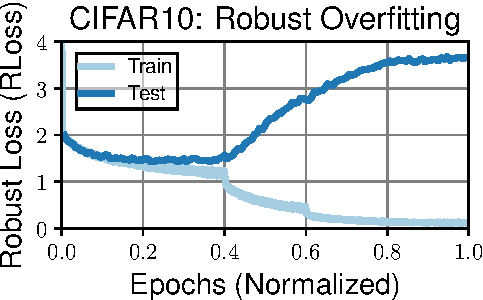
\includegraphics[width=\textwidth]{plots/talk_overfitting13.pdf}
				\end{minipage}
				\hfill
				\begin{minipage}[t]{0.01\textwidth}
					\vspace*{0px}
				
					{\color{black!50!white}\rule{0.5px}{2cm}}
				\end{minipage}
				\hfill
				\begin{minipage}[t]{0.48\textwidth}
					\vspace*{0px}
					
					\footnotesize
					
					\underline{Hypothesis}:\\\emph{Robust overfitting} of adversarial training caused by sharp minima.
				\end{minipage}
				\vspace*{-1px}
			\end{tcolorbox}
			\vspace*{-6px}
			
			\begin{tcolorbox}[
				enhanced,
				boxsep=4pt,
				left=0pt,
				right=0pt,
				top=2pt,
				toptitle=0pt,
				bottomtitle=2pt,
				bottom=0pt,
				colback=white,
				colframe=gray!12!white,
				width=1\textwidth, 
				enlarge left by=0mm,
				arc=0pt,outer arc=0pt,
				boxrule=1pt,
				title=\footnotesize\bfseries Measuring Robust Flatness,
				coltitle=MPIIblack,
				colbacktitle=gray!12!white,
				titlerule style=white,
				collower=MPIIblack,
				]
				\color{MPIIblack}
				\footnotesize
				\vspace*{-7px}
				\begin{center}
					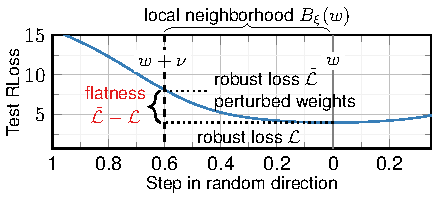
\includegraphics[width=0.75\textwidth]{fig/main_illustration1_4.pdf}
					
					\vspace*{-0.3cm}
					{\color{MPIIgray}\rule{0.9\textwidth}{0.5px}}
				\end{center}
				\vspace*{-0.6cm}
				{\color{MPIIblack}
				\fontsize{6}{8}
				\begin{align}
					\mathbb{E}_{\nu}[\max\limits_{\|\delta\|_\infty \leq \epsilon} \mathcal{L}(f(x{+}\delta; w{+}\nu), y)] - \max\limits_{\|\delta\|_\infty \leq \epsilon} \mathcal{L}(f(x{+}\delta;w), y)\notag
				\end{align}}
				\vspace*{-0.45cm}
			\end{tcolorbox}
		\end{minipage}
		\hfill
		\begin{minipage}[t]{0.49\textwidth}
			\vspace*{0px}
			
			\begin{tcolorbox}[
				enhanced,
				boxsep=4pt,
				left=0pt,
				right=0pt,
				top=2pt,
				toptitle=0pt,
				bottomtitle=2pt,
				bottom=0pt,
				colback=white,
				colframe=gray!12!white,
				width=1\textwidth, 
				enlarge left by=0mm,
				arc=0pt,outer arc=0pt,
				boxrule=1pt,
				title=\footnotesize\bfseries Sharp Minima Cause Robust Overfitting,
				coltitle=MPIIblack,
				colbacktitle=gray!12!white,
				titlerule style=white,
				collower=MPIIblack,
				]
				\color{MPIIblack}
				\footnotesize
				\vspace*{-5px}
				\centering
				\begin{minipage}[t]{0.425\textwidth}
					\begin{tikzpicture}[remember picture]\node[opacity=1] at (0,0) {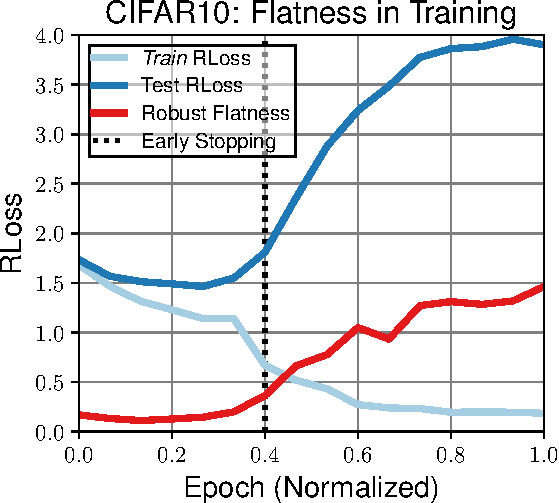
\includegraphics[height=2.5cm]{plots/talk_overview22.pdf}};\end{tikzpicture}
				\end{minipage}
				\begin{minipage}[t]{0.09\textwidth}
					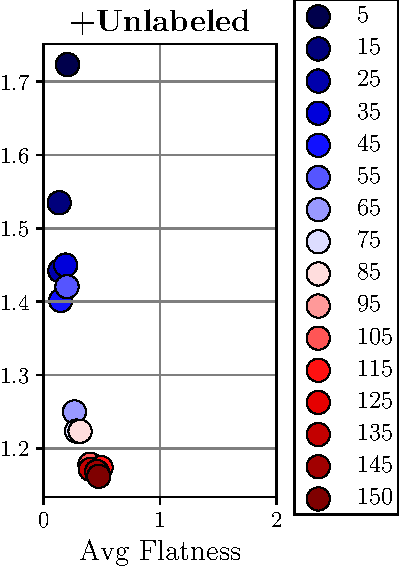
\includegraphics[height=2.5cm,clip,trim={5cm 0cm 0cm 0cm}]{../paper/plots_main_flatness_epochs_correlation_seq_500k.pdf}
				\end{minipage}
				\begin{minipage}[t]{0.275\textwidth}
					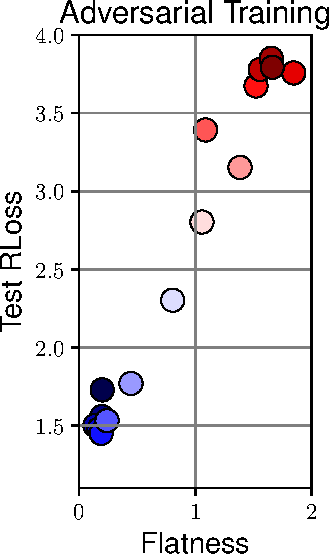
\includegraphics[height=2.5cm]{plots/talk_flatness_epochs_correlation_seq.pdf}
				\end{minipage}
			\end{tcolorbox}
			\vspace*{-6px}
			
			\begin{tcolorbox}[
				enhanced,
				boxsep=4pt,
				left=0pt,
				right=0pt,
				top=2pt,
				toptitle=0pt,
				bottomtitle=2pt,
				bottom=0pt,
				colback=white,
				colframe=gray!12!white,
				width=1\textwidth, 
				enlarge left by=0mm,
				arc=0pt,outer arc=0pt,
				boxrule=1pt,
				title=\footnotesize\bfseries Correlation between Robustness \& Flatness,
				coltitle=MPIIblack,
				colbacktitle=gray!12!white,
				titlerule style=white,
				collower=MPIIblack,
				]
				\color{MPIIblack}
				\footnotesize
				\vspace*{-3px}
				\centering
				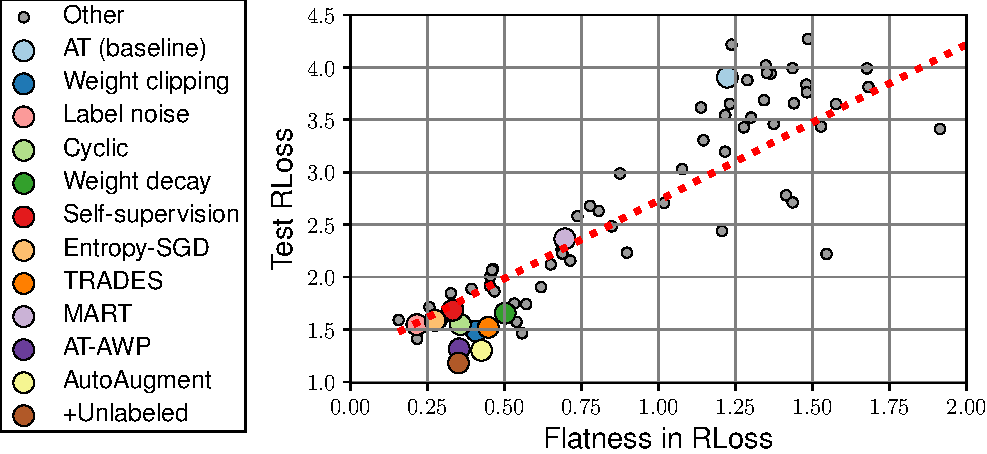
\includegraphics[width=5.5cm]{plots/talk_flatness_correlation_seq_loss.pdf}
			\end{tcolorbox}
		\end{minipage}
		\vspace*{-5px}
		
		\begin{minipage}[t]{0.75\textwidth}
			\vspace*{0px}
			
			\begin{tcolorbox}[
				enhanced,
				boxsep=4pt,
				left=0pt,
				right=0pt,
				top=2pt,
				toptitle=0pt,
				bottomtitle=2pt,
				bottom=0pt,
				colback=gray!12!white,
				colframe=gray!12!white,
				width=1\textwidth, 
				enlarge left by=0mm,
				arc=0pt,outer arc=0pt,
				boxrule=1pt,
				title=,
				coltitle=MPIIblack,
				colbacktitle=gray!12!white,
				titlerule style=white,
				collower=MPIIblack,
				]
				\color{MPIIblack}
				\footnotesize\bfseries More details: \href{https://davidstutz.de/flatness}{\texttt{davidstutz.de/flatness}} {\color{MPIIgray}|} \href{https://arxiv.org/abs/2104.04448}{\texttt{arxiv.org/abs/2104.04448}}
			\end{tcolorbox}
		\end{minipage}
		\hspace*{0.25cm}
		\begin{minipage}[t]{0.2\textwidth}
			\vspace*{2px}
			
			
\includegraphics[height=0.85cm]{Unknown-3}
		\end{minipage}
	\end{frame}
\end{document}
